\documentclass[letterpaper,twocolumn,10pt]{article}
\usepackage{epsfig,xspace,url}
\usepackage{authblk}
\usepackage{graphicx}
\usepackage{listings}
\graphicspath{ {images/} }

\title{Third Party Encrypted Storage}
\author{Travis Taylor, John Robe, and Daniel James}
\affil{School of Computing, University of Utah}

\begin{document}

%Code listing formatting
\lstdefinestyle{codestyle}{
    basicstyle=\footnotesize,
    frame=single,
    breaklines=true
}
\lstset{style=codestyle}


\maketitle

\section{Introduction}

Remembering a good password is hard. Unsurpsingly most people take the path of least resistence, and simply don't use good passwords. Frequently user passwords consist of personal information or absolutely simple ones to guess like \textit{1234}\cite{easypass}. Many organizations require that you use certain combinations of letters, numbers, and symbols. This frequently annoys users, as it makes passwords more difficult to use. Given this constraint on passwords, many users make one password that will satisfy many of the complexity requirements for most passwords, and simply use that everywhere. This is possibly worse than a simple password, as once one of those are compromised, and this happens with somewhat alarming frequency\cite{databreach}, the attacker has access to all of your other accounts.

There are a few current solutions to this. One of the most common allows you to log in to services using an API provided by many commonly used services like Facebook, Google, and Twitter. This requires integration on the services part to use the third party API. This presents a new problem, now those third-party services have all your information about what services you use, as well as holding a lot of Personal Identifiable information (PII). Many users don't like the idea of these third-party services having so much personal information about them, and thus don't even use them, or don't want to use them to log into other services.


\section{Design}

Our solution to this problem is to not use passwords at all. In a sentence, instead of the users remembering passwords, the device the user uses does for him. Since a computer doesn't have the memory limitations a human does, it can have absolutely random passwords of sufficiently large length.

See figure \ref{design}.

Our basic design consists of four entities
\begin{itemize}
    \item \textbf{User} - The user that desires to use our application, to store their data securely
    \item \textbf{Authentication Server} - The server that will store the encrypted data for the user, without having the key.
    \item \textbf{Portal Application} - This is the application that retrieves data from the user to unlock the data on the authentication server.
    \item \textbf{Demo Application} - This application is the entity that requests data about the user.
\end{itemize}

\begin{figure*}[ht]
\centering
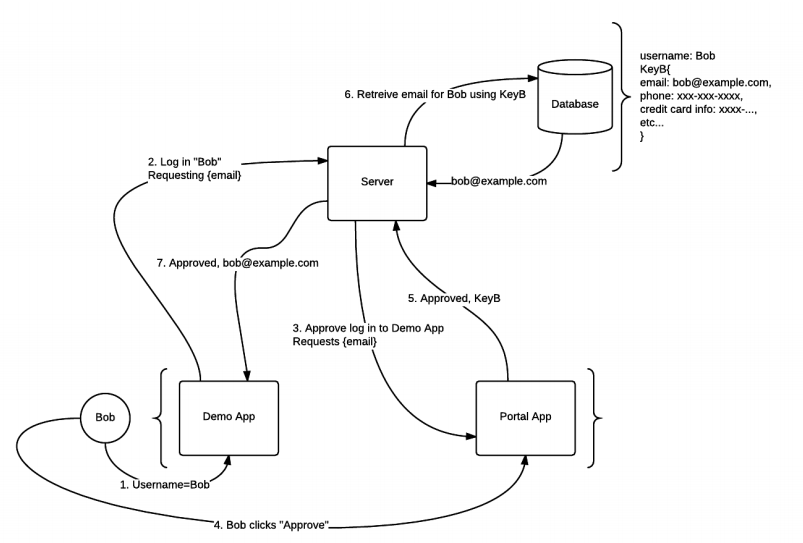
\includegraphics[width=\textwidth]{Design}
\caption{Overall system design}
\label{design}
\end{figure*}



\section{Implemention}
%TODO Probably add more here between the example run through and the first sentence
    We chose to write our demo application in three parts: the server, the portal, and the demo application. An example run through of our application would like like so:
\begin{figure}[ht]
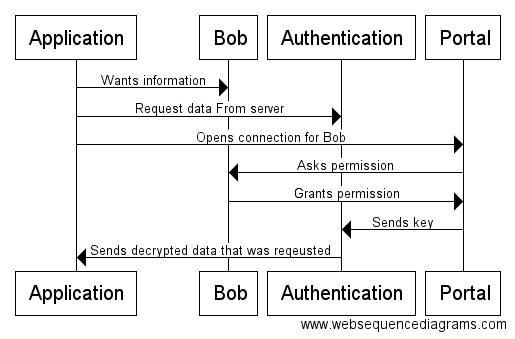
\includegraphics[width=0.45\textwidth]{messageDiagram}
\caption{Message Flow}
\end{figure}

\paragraph{RPCs and Message Formats}
    We chose to use Thrift\cite{thrift} as our RPC\footnote{remote procedure call} and message formatting framework. We chose this primarily because it allows for multiple different output languages from it's initial IDL\footnote{interface definition language}. The way Thrift works is you define a set of structures and functions in an IDL, and then compile it to the various langauges you wish to use it in. A snippet of our Thrift IDL file:

\begin{minipage}{\linewidth}
\lstinputlisting[firstline=0,lastline=22]{../thrift/cs5490.thrift}
\end{minipage}

\subsection{Authentication Server}
    The authentication server deals with holding the encrypted data. It is relatively simple, as it merely has to hold a 2 column table, and provide the ability to decrypt with a given key. The server provides this functionality through Apache Thrift\cite{thrift}. It provides some simple functions:
    \begin{itemize}
        \item \textbf{createAccount} - Creates the account for the user, and generates the key for it.
        \item \textbf{requestPermission} - The application requesting access will call this function with the requested data fields and user.
        \item \textbf{checkForPermissionRequest} - Portal can check if it has any pending reqeusts\footnote{In lieu of push notifications, we moved for polling due to time constraints} 
        \item \textbf{decideRequest} - Once the user decides what they want to do, the portal application will call this with the decision and, if in the affirmative, the key.
        \item \textbf{checkForPermissionGranted} - The demo application can poll with a requerst ID to see if their request has been confirmed or denied.
    \end{itemize}

The backend storage is SQLite, given the simple nature of the data. This could have also been done in a key-value pair database, however, that would have required setting up another server for this.
\subsection{Portal Application}
\subsection{Demo Application}

\section{Alterative Methods}

Talk about how we could have done a few things differently, like having the portal generate the key and then send it to the server, as this would have allowed it to generate it from a password and not have to even talk to the server.


{
    \small
    \bibliographystyle{acm}
    \bibliography{biblio}
}

\end{document}
